\newcommand{\fancyrisklattice}
{
\setlength{\unitlength}{1.7pt}

%\begin{center}
\begin{picture}(40,19)
\thicklines
\put(7,4){\line(1,1){10}}
\put(17,-13){\line(-1,1){10}}
\put(33,4){\line(-1,1){10}}
\put(23,-13){\line(1,1){10}}
\put(5,8){$\po$}
\put(5,-9){$\po$}
\put(30,8){$\po$}
\put(30,-9){$\po$}
\put(16,16){$\mathit{high}$}
\put(-3,-1){$\mathit{medium}$}
\put(25,-1){$\mathit{moderate}$}
\put(15,-18){$\mathit{low}$}
\end{picture}
%\end{center}
\vspace{10mm}
}

\newcommand{\risklattice}
{
\setlength{\unitlength}{1.7pt}

%\begin{center}
\begin{picture}(40,19)
\thicklines
\put(7,4){\vector(1,1){10}}
\put(17,-13){\vector(-1,1){10}}
\put(33,4){\vector(-1,1){10}}
\put(23,-13){\vector(1,1){10}}
\put(15,16){$\mathit{high}$}
\put(-3,-1){$\mathit{medium}$}
\put(25,-1){$\mathit{moderate}$}
\put(15,-18){$\mathit{low}$}
\end{picture}
%\end{center}
\vspace{10mm}
}

\newcommand{\rmemfig}
{
\begin{fpfig*}[t]{$\RTR$ semantic functions}{figure-rmem}
\begin{eqnarray*}
%\bounds_\thresh[\rmem](A.r) &=& \setdefn{(B,\risk)\ \mid\ (B,\risk) \in \bounds[\rmem](A.r) \text{\ and\ } \risk \po \thresh(A.r)}\\[4mm]
\bounds[\rmem](A.r) &=& \biguplus\limits_{\cred{A.r}{e}{\risk} \in \creds} 
\expr[\rmem](e) \riskplus \risk \\[4mm]
\expr[\rmem](B) &=& \setdefn{(B,\bot)}\\
\expr[\rmem](A.r)&=& \rmem(A.r)\\
\expr[\rmem](A.r_1.r_2) &=& \biguplus\limits_{(B,\risk)\in \rmem(A.r_1)}
  \rmem(B.r_2) \linkplus \risk \\
\expr[\rmem](f_1 \cap \cdots \cap f_n) &=&
   \bigotimes\limits_{1\le i \le n} \expr[\rmem](f_i)
\end{eqnarray*}
\end{fpfig*}
}

\newcommand{\discoveryexamplefig}
{
\begin{fpfig*}{Graphical Example of $\checkmem$ Execution}{figure-discovery-example}
\vspace{3mm}
\hspace{2mm}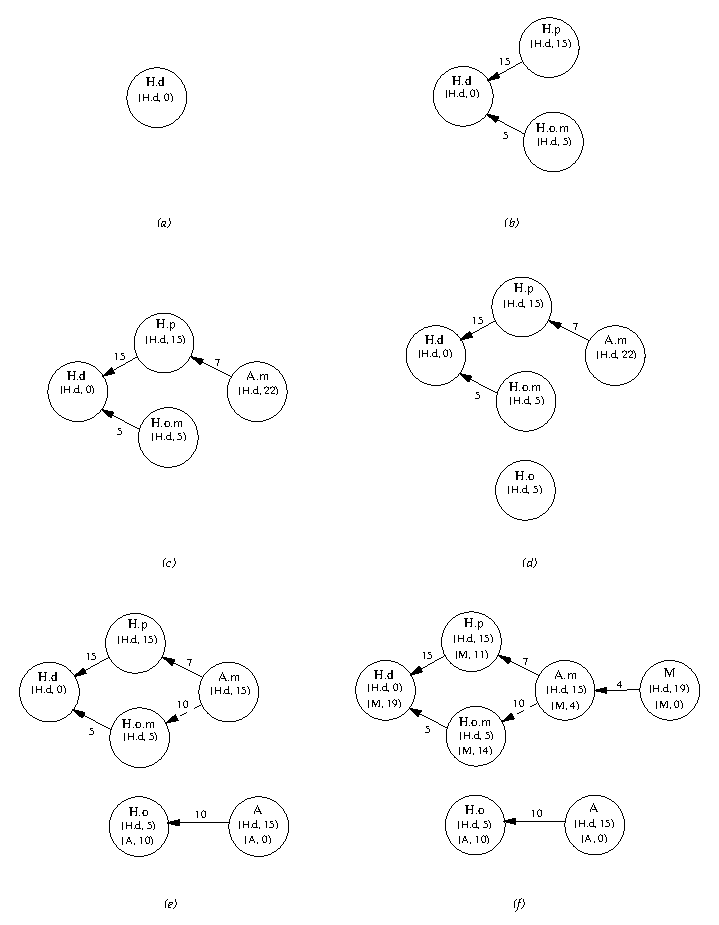
\includegraphics{discovery}
\vspace{2mm}
\end{fpfig*}
}